\chapter{Экспериментальное исследование параметров устройства квантовой коммуникации с недоверенным приемным узлом} \label{ch:ch5}
\section{Интерференция сигналов на боковых частотах фазомодулированного излучения} \label{sec:ch5/sec1}


 \begin{figure}[ht]
  \centering
  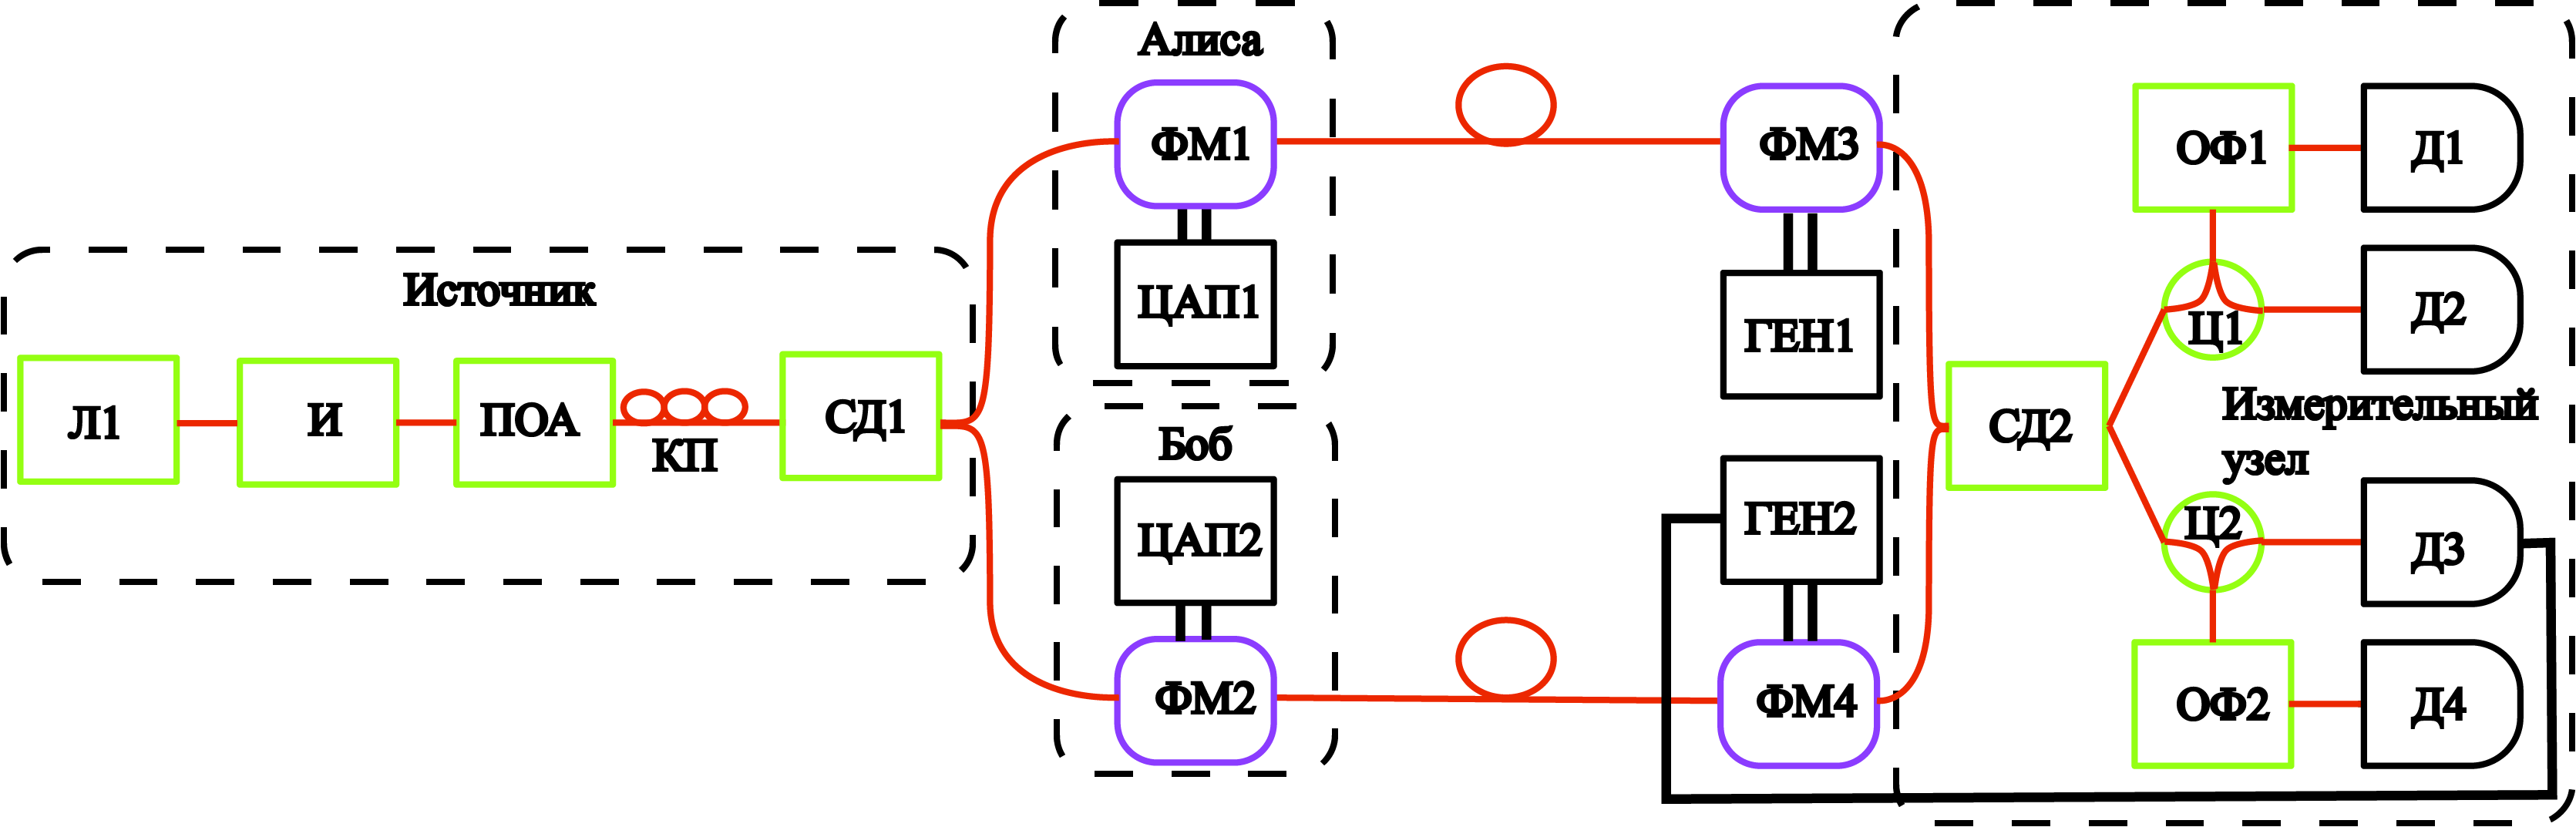
\includegraphics[scale=0.5]{Scheme_colored_rus.png}
  \caption{Принципиальная схема экспериментального стенда}
  \label{fig:RF_sin}
\end{figure}

\pagebreak

%%%%%%%%%%%%%%%%%%%%%%%%%%%%%%%%%%%%%%%%%%%%%%%%%%%%%%%%%%%%%%%%%%%%%%%%%%%%%%%%%
\section{Характеристики компонентов экспериментального стенда} \label{ch:ch5/sec2}

 \begin{figure}[ht]
  \centering
  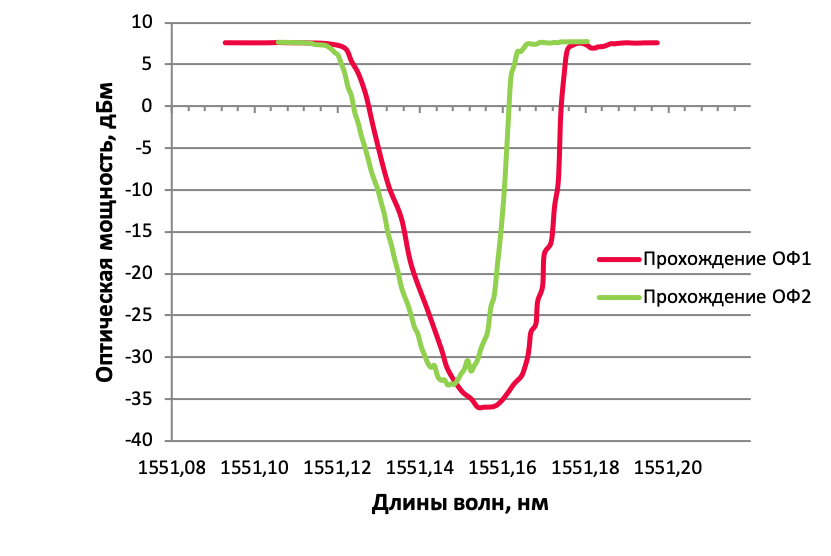
\includegraphics[scale=0.8]{T-spectrums.png}
  \caption{Спектральные характеристики оптических фильтров}
  \label{fig:Spectrums}
\end{figure}

\pagebreak

%%%%%%%%%%%%%%%%%%%%%%%%%%%%%%%%%%%%%%%%%%%%%%%%%%%%%%%%%%%%%%%%%%%%%%%%%%%%%%%%%%%%%%%%%%%%%%%%%%%%%%%%%%%%%%%%%
\section{Экспериментальный стенд} \label{ch:ch5/sec3}

 \begin{figure}[ht]
  \centering
	 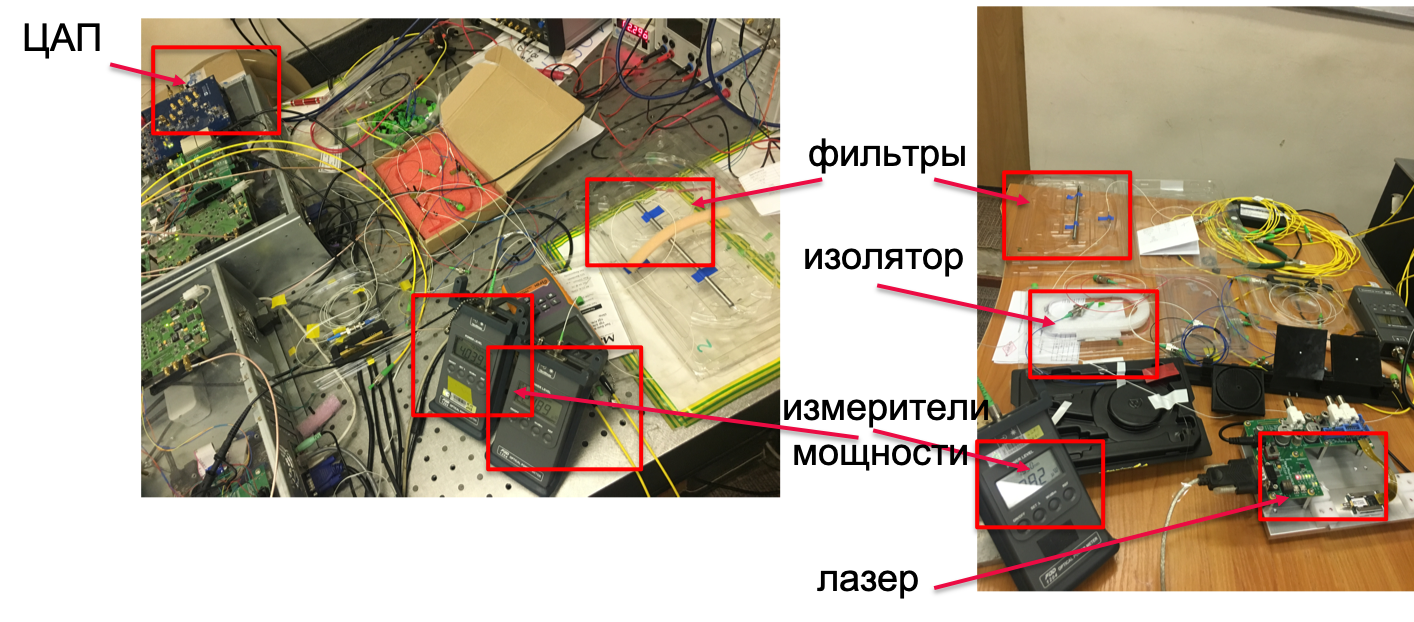
\includegraphics[scale=0.7]{Experimental_setup_TF}
  \caption{Фотография экспериментального стенда}
  \label{fig:experimental_setup_TF}
\end{figure}

\pagebreak

%%%%%%%%%%%%%%%%%%%%%%%%%%%%%%%%%%%%%%%%%%%%%%%%%%%%%%%%%%%%%%%%%%%%%%%%%%%%%%%%%%%%%%%%%%%%%%%%%%%%%%%%%%%%%%%%%
\section{Зависимость интенсивности на боковых частотах от сдвига фаз в результате интерференции в классическом режиме} \label{ch:ch5/sec4}

 \begin{figure}[ht]
  \centering
  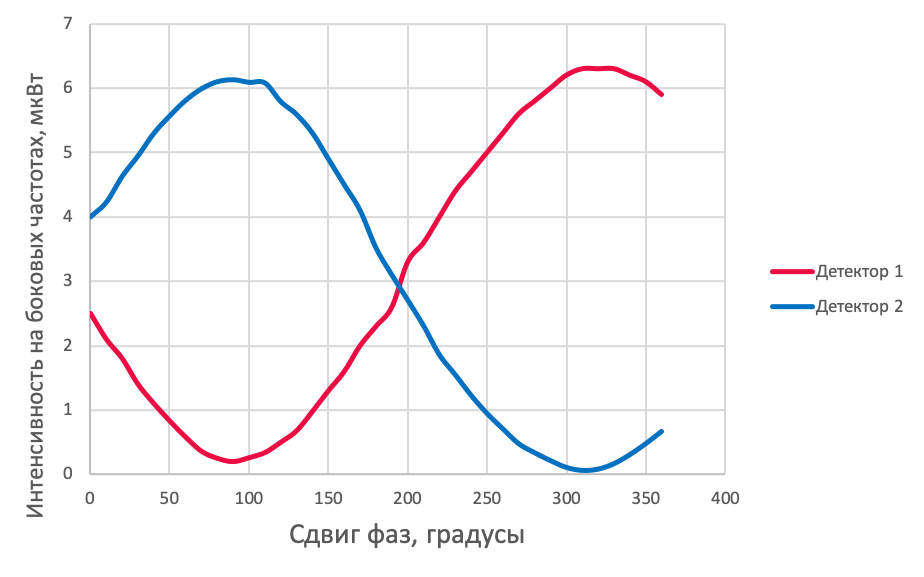
\includegraphics[scale=0.7]{Experimental_TF_classical.png}
  \caption{Зависимость интенсивности на боковых частотах в результате интерференции от разности фаз модулирующих сигналов}
  \label{fig:Experimental_TF_classical}
\end{figure}

\pagebreak

%%%%%%%%%%%%%%%%%%%%%%%%%%%%%%%%%%%%%%%%%%%%%%%%%%%%%%%%%%%%%%%%%%%%%%%%%%%%%%%%%%




\section{Вероятности срабатываний детекторов} \label{ch:ch5/sec5}

 Известно, что оптический фильтр отражает центральную оптическую моду ($k=0$). Значит, среднее число фотоном на входе в каждый детектор может быть найдена как \ref{nph1}. 
 
\begin{align}\label{nph1}
    n(\Delta\varphi)_{1,2}&=\mu_0\eta_c\Bigg(\sum_{k\neq 0}|d_{0k}^{S}(\beta)|^2 + \vartheta|d_{0k}^{S}(\beta)|^2 \pm \nonumber \\
    &\pm \cos(\varphi_0)\Big(\sum_{k\neq 0}|d_{0k}^{S}(\beta)|^2e^{i\Delta\varphi k}+ \vartheta|d_{0k}^{S}(\beta)|^2 \Big) \Bigg),
\end{align}

где $\Delta\varphi=\varphi_B-\varphi_A$, $\varphi_0$ это относительная оптическая фаза между импульсами отправителя (Алисы) и получателя (Боб), $\vartheta \ll 1$ часть центральной моды ($k=0$) проходящая через фильтр, ввиду ограниченности его характеристики. Используя свойства d-функци из \cite{varshalovich1988quantum}, можно упростить предыдущее выражение \ref{nph}

\begin{align}
    n(\Delta\varphi)_{1,2}=\mu_0\eta_c\Big(1-(1-\vartheta)(1\mp\cos(\varphi_0))|d_{00}^{S}(\beta)|^2 \pm \nonumber \\
    \pm\cos(\varphi_0)d_{00}^{S}(\beta')\Big) \label{nph},
\end{align}

где аргумент $\beta'$ получен следующим образом \ref{betaappox}. 

\begin{equation} \label{betaappox}
    \cos(\beta')=\cos^2(\beta) \mp \sin^2(\beta)\cos(\Delta\varphi).
\end{equation}

Чтобы оценить вероятность срабатывания воспользуемся линейным приближением Манделя, предполагая слабые интенсивности ($n(\Delta\varphi)_{1,2} \ll 1$):

\begin{eqnarray}
    \mathcal{P}_{1,2}^{+}(\Delta\varphi)=\left(n(\Delta\varphi)_{1,2}\eta_DF+\gamma_{dark}\right)\Delta t, \label{pdet}
\end{eqnarray}

где $\eta_D$ квантовая эффективность, $F$ частота смены состояний, $\gamma_{dark}$ частота темновых отсчетов детектора одиночных фотонов, и $\Delta t$ время окна срабатывания. Для простоты положим $\Delta t F=1$. Отсутствие срабатывания определим, как $\mathcal{P}_{1,2}^{-}(\Delta\varphi)=1-\mathcal{P}_{1,2}^{+}(\Delta\varphi)$.     


Используем несколько полезных приближений, которые помогут оценить квантовый коэффициент ошибок по битам (QBER) и скорости формирования просеянного ключа. Для начала положим, что число взаимодействующих мод велико ($S\rightarrow \infty$), что действительно так для стандартных волоконно-оптических модуляторов. Тогда можно использовать приближение d-функций следующим образом:

\begin{align}
d_{nk}^S(\beta) &\xrightarrow{S\rightarrow \infty} J_{n-k}(m), \label{limdj} \\
\beta &\propto m, \label{propto}
\end{align}
где $J_k(m)$ функция Бесселя первого порядка. Полагая значение $m$ малым, что действительно так, в соотвествии с теорией классической модуляции воспользуемся приближением первого порядка функции Бесселя. 


Так в соответствии с уравнение \ref{betam} $\beta \rightarrow 0$, следовательно можно использовать аппроксимации первого порядка для выражения \ref{betaappox} в терминах $m$ подразумевая пропорциональность в уравнении \ref{propto}.


Определим уравнение~\ref{pdet} следующим образом:

\begin{align}\label{pdet1}
 \mathcal{P}_{1,2}^{+}(\Delta\varphi)&=\mu\eta\Big(1\pm\cos(\Delta\varphi)\cos(\varphi_0)\Big)+ \nonumber
 \\
 &+\vartheta\Big(\mu_c\eta(1\pm\cos(\varphi_0))\Big)+p_{dark},
\end{align}


где $\eta$ полная оптическая пропускная способность квантового канала с учетом квантовой эффективности детектора, $p_{dark}=\gamma_{dark}\Delta t$ это вероятность темнового срабатывания во временном интервале $\Delta t$, и $\mu$ и $\mu_c$ это среднее число фотонов на боковых и на центральной моде соотвественно после модуляции, как определено:

\begin{align}
    \mu&=\mu_0\sum_{k\neq 0}|d_{0k}^{S}(\beta)|^2, \\
    \mu_c&=\mu_0-\mu=\mu_0(1-\sum_{k\neq 0}|d_{0k}^{S}(\beta)|^2).
\end{align}
Выраение в уравнени~\ref{pdet1} даёт точное соотношение между экспериментальными параметрами и показывает, как они влияют на вероятности детектирования квантовых состояний. 


\pagebreak

%%%%%%%%%%%%%%%%%%%%%%%%%%%%%%%%%%%%%%%%%%%%%%%%%%%%%%%%%%%%%%%%%%%%%%%%%%%%%%%%%%
\section{Зависимость интенсивности на боковых частотах от сдвига фаз в результате интерференции в режиме счета фотонов} \label{ch:ch5/sec6}


 \begin{figure}[ht]
  \centering
  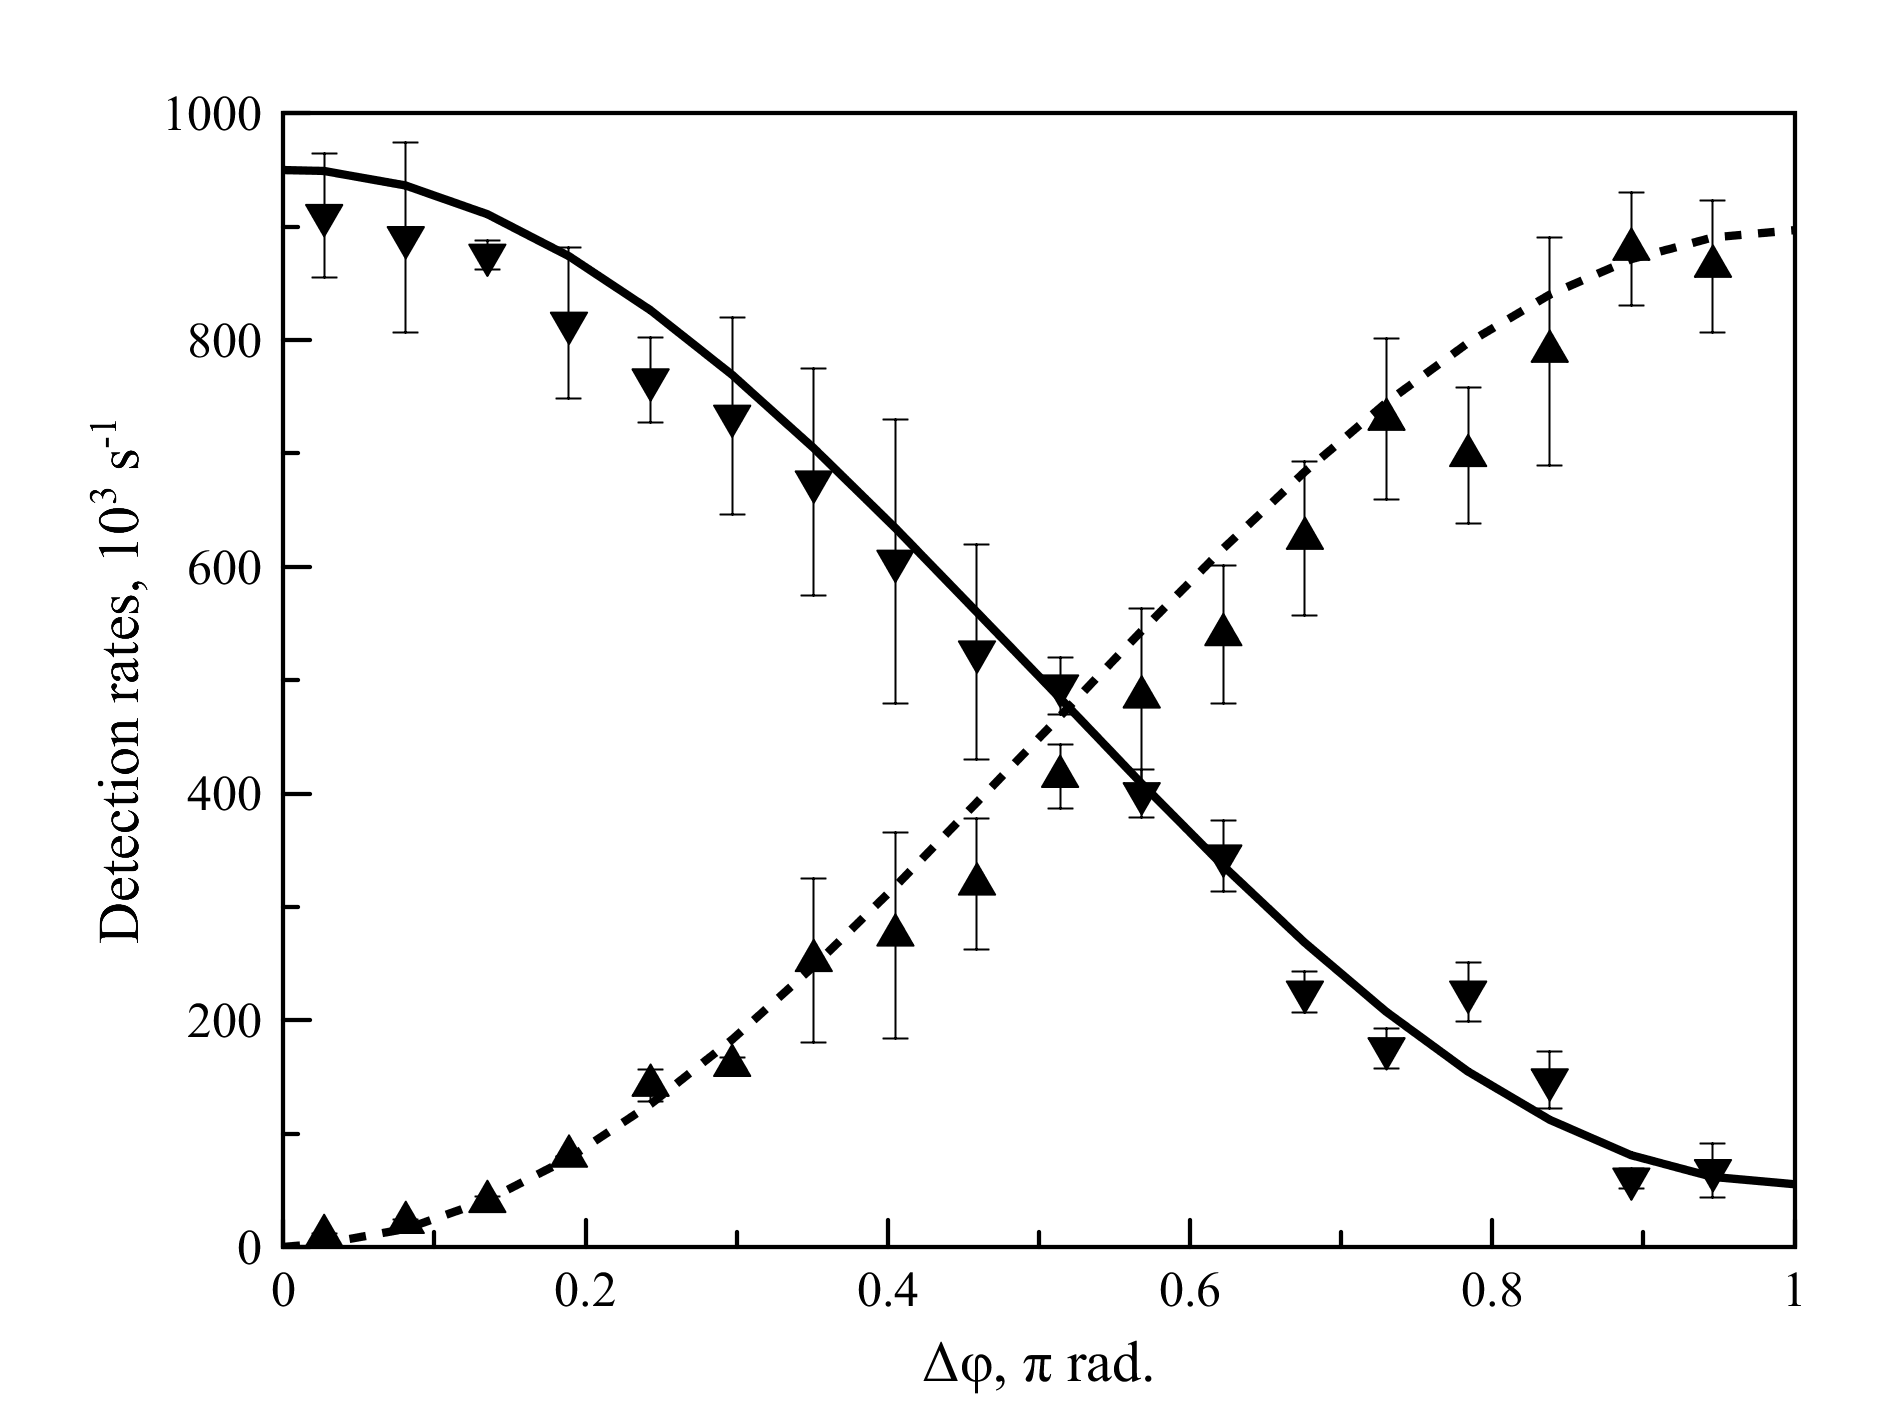
\includegraphics[scale=0.2]{ExperimentTF.png}
  \caption{Зависимость количества отсчетов в результате интерференции от разности фаз модулирующих сигналов}
  \label{fig:Experimental_TF}
\end{figure}


\pagebreak

%%%%%%%%%%%%%%%%%%%%%%%%%%%%%%%%%%%%%%%%%%%%%%%%%%%%%%%%%%%%%%%%%%%%%%%%%%%%%%%%%%
\section{Оценка коэффициента битовых ошибок и скорости формирования ключа} \label{ch:ch5/sect7}

Далее рассмотрим только те случаи, где срабатывание происходит только на одном из детекторов в единицу времени.  Таким образом, вероятности срабатываний $R$ определяются как:

\begin{align}
    R&=\Big(\mathcal{P}_{1}^{+}\mathcal{P}_{2}^{-}(\Delta\varphi=\varphi_m)+\mathcal{P}_{1}^{-}\mathcal{P}_{2}^{+}(\Delta\varphi=\pi+\varphi_m)+ \nonumber \\
    &+\mathcal{P}_{1}^{+}\mathcal{P}_{2}^{-}(\Delta\varphi=\pi+\varphi_m)+\mathcal{P}_{1}^{-}\mathcal{P}_{2}^{+}(\Delta\varphi=\varphi_m)\Big),
\end{align}


где $\varphi_m$ средняя величина несоответствия фаз $\varphi_A$ и $\varphi_B$. Первые два слагаемых - это вероятности успешного определения битов легитимными пользователями, тогда как оставшиеся два слагаемых - вероятности смены бита на противоположный (bitflip) (полагая $\varphi_0 \approx 0$). Таким образом, можно определить выражение для QBER $Q$ следующим образом:

\begin{align}
    Q=\frac{\mathcal{P}_{1}^{-}\mathcal{P}_{2}^{+}(\Delta\varphi=\varphi_m)+\mathcal{P}_{1}^{+}\mathcal{P}_{2}^{-}(\Delta\varphi=\pi+\varphi_m)}{R}.
\end{align}


Наконец, можно определить выражение для оценки среднего значения скорости формирования просеянного ключа $K$ (одинаковые биты между легитимными пользователями, но коррелирующие с возможным результатом у злоумышленника, что требуется проведения процедуры усиления секретности)
\begin{equation}
    K=FR(1-h(Q)),
\end{equation}
где $h(Q)$ это функция двоичной энтропии. 

\pagebreak

%%%%%%%%%%%%%%%%%%%%%%%%%%%%%%%%%%%%%%%%%%%%%%%%%%%%%%%%%%%%%%%%%%%%%%%%%%%%%%%%%%
\section{Выводы по главе} \label{ch:ch5/sec8}


В \ref{ch:ch5} главе показано, что в результате интерференции квантового фазомодулированного сигнала на боковых частотах на симметричном светоделителе в схеме квантовой рассылки ключа с узлом регистрации, независящим от легитимного пользователя, происходит спектральное разделение квантового сигнала и сигнала на центральной длине волны с их независимой регистрацией в разных плечах светоделителя. 

\pagebreak
